% =========================================================================
% BÀI 14: KHỐI LẬP PHƯƠNG, KHỐI HỘP CHỮ NHẬT (CHỦ ĐỀ 4 - TOÁN LỚP 1)
% TOÀN BỘ CÂU HỎI ĐƯỢC VẼ HÌNH MINH HỌA TRỰC QUAN 100% BẰNG TIKZ 3D
% =========================================================================

% --- CÁC HÀM VẼ KHỐI 3D TRỰC QUAN CHO HỌC SINH LỚP 1 ---

% 1. Khối lập phương 3D
\providecommand{\VeKhoiLapPhuong}[4][yellow!60]{% #1=màu, #2=x, #3=y, #4=cạnh
  \begin{scope}[shift={(#2,#3)}]
    \pgfmathsetmacro{\s}{#4}
    \pgfmathsetmacro{\dx}{\s*0.42}
    \pgfmathsetmacro{\dy}{\s*0.32}
    % Mặt trước
    \draw[fill=#1, draw=black!75, line width=1.1pt] (0,0) rectangle (\s,\s);
    % Mặt trên
    \draw[fill=white!35!#1, draw=black!75, line width=1.1pt] (0,\s) -- (\s,\s) -- (\s+\dx,\s+\dy) -- (\dx,\s+\dy) -- cycle;
    % Mặt phải
    \draw[fill=black!25!#1, draw=black!75, line width=1.1pt] (\s,0) -- (\s+\dx,\dy) -- (\s+\dx,\s+\dy) -- (\s,\s) -- cycle;
  \end{scope}
}

% 2. Khối hộp chữ nhật 3D
\providecommand{\VeKhoiHopChuNhat}[6][cyan!50]{% #1=màu, #2=x, #3=y, #4=rộng, #5=cao, #6=sâu
  \begin{scope}[shift={(#2,#3)}]
    \pgfmathsetmacro{\w}{#4}
    \pgfmathsetmacro{\h}{#5}
    \pgfmathsetmacro{\dx}{#6*0.42}
    \pgfmathsetmacro{\dy}{#6*0.32}
    % Mặt trước
    \draw[fill=#1, draw=black!75, line width=1.1pt] (0,0) rectangle (\w,\h);
    % Mặt trên
    \draw[fill=white!35!#1, draw=black!75, line width=1.1pt] (0,\h) -- (\w,\h) -- (\w+\dx,\h+\dy) -- (\dx,\h+\dy) -- cycle;
    % Mặt phải
    \draw[fill=black!25!#1, draw=black!75, line width=1.1pt] (\w,0) -- (\w+\dx,\dy) -- (\w+\dx,\h+\dy) -- (\w,\h) -- cycle;
  \end{scope}
}

% 3. Viên xúc xắc 3D
\providecommand{\VeVienXucXac}[2]{% #1=x, #2=y
  \begin{scope}[shift={(#1,#2)}]
    % Mặt trước (2 chấm)
    \draw[fill=white, draw=gray!85!black, line width=1.2pt, rounded corners=1.5pt] (0,0) rectangle (1.2,1.2);
    \fill[black] (0.35,0.35) circle (0.08cm);
    \fill[black] (0.85,0.85) circle (0.08cm);
    % Mặt trên (1 chấm đỏ ở giữa)
    \draw[fill=gray!12, draw=gray!85!black, line width=1.2pt] (0,1.2) -- (1.2,1.2) -- (1.65,1.55) -- (0.45,1.55) -- cycle;
    \fill[red!85!black] (0.85,1.38) circle (0.1cm);
    % Mặt phải (3 chấm)
    \draw[fill=gray!28, draw=gray!85!black, line width=1.2pt] (1.2,0) -- (1.65,0.35) -- (1.65,1.55) -- (1.2,1.2) -- cycle;
    \fill[black] (1.35,0.3) circle (0.065cm);
    \fill[black] (1.43,0.78) circle (0.065cm);
    \fill[black] (1.52,1.26) circle (0.065cm);
  \end{scope}
}

% 4. Khối Rubik 3D
\providecommand{\VeKhoiRubik}[2]{% #1=x, #2=y
  \begin{scope}[shift={(#1,#2)}, scale=0.75]
    % Mặt trước (đỏ)
    \foreach \i in {0,1,2} {
      \foreach \j in {0,1,2} {
        \draw[fill=red!85!black, draw=black, line width=0.8pt] (\i*0.48,\j*0.48) rectangle (\i*0.48+0.46,\j*0.48+0.46);
      }
    }
    % Mặt trên (vàng)
    \foreach \i in {0,1,2} {
      \foreach \j in {0,1,2} {
        \draw[fill=yellow!90!orange, draw=black, line width=0.8pt] 
          (\i*0.48+\j*0.2, 1.44+\j*0.15) -- (\i*0.48+\j*0.2+0.46, 1.44+\j*0.15) -- 
          (\i*0.48+\j*0.2+0.66, 1.44+\j*0.15+0.15) -- (\i*0.48+\j*0.2+0.2, 1.44+\j*0.15+0.15) -- cycle;
      }
    }
    % Mặt phải (xanh dương)
    \foreach \i in {0,1,2} {
      \foreach \j in {0,1,2} {
        \draw[fill=blue!85!black, draw=black, line width=0.8pt] 
          (1.44+\i*0.2, \j*0.48+\i*0.15) -- (1.44+\i*0.2+0.2, \j*0.48+\i*0.15+0.15) -- 
          (1.44+\i*0.2+0.2, \j*0.48+\i*0.15+0.61) -- (1.44+\i*0.2, \j*0.48+\i*0.15+0.46) -- cycle;
      }
    }
  \end{scope}
}

% =========================================================================
% PHẦN 1: TRẮC NGHIỆM LỰA CHỌN (12 CÂU)
% =========================================================================
\textbf{Phần 1. Trắc nghiệm lựa chọn}
\setcounterpageref{ex}{0}

% --- CÂU 1 ---
\begin{ex} %[1H4N14]
Trong các đồ vật dưới đây, đồ vật nào có dạng \textbf{khối lập phương}?
\begin{center}
\setlength{\tabcolsep}{10pt}
\begin{tabular}{cccc}
  \begin{tikzpicture}[scale=0.65]
    \VeKhoiHopChuNhat[magenta!40]{-0.9}{-0.6}{1.8}{1.0}{0.8}
    \node[below=3pt, font=\scriptsize\bfseries\color{purple!80!black}] at (0,-0.6) {Hộp bánh};
  \end{tikzpicture}
  &
  \begin{tikzpicture}[scale=0.65]
    \VeVienXucXac{-0.8}{-0.6}
    \node[below=3pt, font=\scriptsize\bfseries\color{red!85!black}] at (0,-0.6) {Viên xúc xắc};
  \end{tikzpicture}
  &
  \begin{tikzpicture}[scale=0.65]
    \shade[ball color=orange!90!white] (0,0.1) circle (0.75cm);
    \node[below=3pt, font=\scriptsize\bfseries\color{orange!90!black}] at (0,-0.6) {Quả bóng};
  \end{tikzpicture}
  &
  \begin{tikzpicture}[scale=0.65]
    \draw[fill=green!35, draw=green!70!black, line width=1pt] (-0.5,-0.5) rectangle (0.5,0.7);
    \draw[fill=green!25, draw=green!70!black, line width=1pt] (0,0.7) ellipse (0.5cm and 0.2cm);
    \draw[fill=green!45, draw=green!70!black, line width=1pt] (0,-0.5) ellipse (0.5cm and 0.2cm);
    \node[below=3pt, font=\scriptsize\bfseries\color{green!70!black}] at (0,-0.6) {Lon nước};
  \end{tikzpicture}
\end{tabular}
\end{center}
\choice
{Hộp bánh quy}
{\True Viên xúc xắc}
{Quả bóng}
{Lon nước ngọt}
\loigiai{
Viên xúc xắc có 6 mặt vuông bằng nhau nên có dạng \textbf{khối lập phương}.\\
\textbf{Đáp án của câu hỏi là B}
}
\end{ex}

% --- CÂU 2 ---
\begin{ex} %[1H4N14]
Hộp quà sinh nhật dưới đây có dạng hình khối gì?
\begin{center}
\begin{tikzpicture}[scale=0.85, baseline=(current bounding box.center)]
  \VeKhoiHopChuNhat[yellow!60]{-1.4}{-0.6}{2.4}{1.2}{1.0}
  \draw[line width=2pt, red!85!black] (-0.2,-0.6) -- (-0.2,0.6) -- (0.22,0.92);
  \draw[line width=2pt, red!85!black] (-1.4,0) -- (1.0,0) -- (1.42,0.32);
  \fill[red!85!black] (0.22,0.92) circle (0.1cm);
  \draw[line width=1.4pt, red!85!black] (0.22,0.92) to[out=135,in=45] (-0.1,1.15) to[out=-135,in=-45] (0.22,0.92);
  \draw[line width=1.4pt, red!85!black] (0.22,0.92) to[out=45,in=135] (0.54,1.15) to[out=-45,in=-135] (0.22,0.92);
  \node[below=4pt, font=\small\bfseries\color{orange!90!black}] at (0,-0.6) {Hộp quà sinh nhật};
\end{tikzpicture}
\end{center}
\choice
{Khối lập phương}
{\True Khối hộp chữ nhật}
{Khối cầu}
{Khối trụ}
\loigiai{
Hộp quà có các mặt là hình chữ nhật nên có dạng \textbf{khối hộp chữ nhật}.\\
\textbf{Đáp án của câu hỏi là B}
}
\end{ex}

% --- CÂU 3 ---
\begin{ex} %[1H4H14]
Khối lập phương dưới đây có bao nhiêu mặt phẳng?
\begin{center}
\begin{tikzpicture}[scale=0.85, baseline=(current bounding box.center)]
  \VeKhoiLapPhuong[cyan!50]{-0.7}{-0.7}{1.4}
  \node[font=\footnotesize\bfseries\color{blue!90!black}] at (0,0) {Mặt trước};
  \node[font=\footnotesize\bfseries\color{blue!80!black}] at (0.3,0.95) {Mặt trên};
  \node[font=\footnotesize\bfseries\color{blue!95!black}, rotate=35] at (1.0,0.2) {Mặt phải};
\end{tikzpicture}
\end{center}
\choice
{$4$ mặt}
{$8$ mặt}
{\True $6$ mặt vuông bằng nhau}
{$12$ mặt}
\loigiai{
Khối lập phương có \textbf{6 mặt} đều là các hình vuông bằng nhau.\\
\textbf{Đáp án của câu hỏi là C}
}
\end{ex}

% --- CÂU 4 ---
\begin{ex} %[1H4H14]
Khối hộp chữ nhật dưới đây có bao nhiêu mặt?
\begin{center}
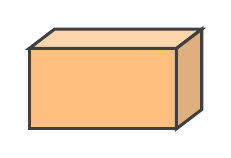
\begin{tikzpicture}[scale=0.85, baseline=(current bounding box.center)]
  \VeKhoiHopChuNhat[orange!50]{-1.2}{-0.6}{2.2}{1.2}{0.9}
\end{tikzpicture}
\end{center}
\choice
{$4$ mặt}
{\True $6$ mặt}
{$8$ mặt}
{$10$ mặt}
\loigiai{
Khối hộp chữ nhật có \textbf{6 mặt}.\\
\textbf{Đáp án của câu hỏi là B}
}
\end{ex}

\newpage
% --- CÂU 5 ---
\begin{ex} %[1H4H14]
Đồ chơi khối rubik $3 \times 3$ dưới đây có dạng hình khối nào?
\begin{center}
\begin{tikzpicture}[scale=0.85, baseline=(current bounding box.center)]
  \VeKhoiRubik{-0.8}{-0.8}
  \node[below=4pt, font=\small\bfseries\color{blue!90!black}] at (0.2,-0.8) {Khối rubik};
\end{tikzpicture}
\end{center}
\choice
{Khối hộp chữ nhật}
{Khối trụ}
{\True Khối lập phương}
{Khối cầu}
\loigiai{
Khối rubik có dạng \textbf{khối lập phương}.\\
\textbf{Đáp án của câu hỏi là C}
}
\end{ex}

% --- CÂU 6 ---
\begin{ex} %[1H4H14]
Bao diêm dưới đây có dạng hình khối gì?
\begin{center}
\begin{tikzpicture}[scale=0.85, baseline=(current bounding box.center)]
  \VeKhoiHopChuNhat[yellow!60]{-1.3}{-0.5}{2.3}{1.0}{0.9}
  \node[font=\footnotesize\bfseries\color{red!85!black}] at (-0.15,0) {DIÊM THỐNG NHẤT};
  \draw[fill=brown!60!black] (1.0,-0.5) -- (1.38,-0.22) -- (1.38,0.78) -- (1.0,0.5) -- cycle;
  \node[below=4pt, font=\small\bfseries\color{brown!80!black}] at (0,-0.5) {Hộp bao diêm};
\end{tikzpicture}
\end{center}
\choice
{\True Khối hộp chữ nhật}
{Khối lập phương}
{Hình tròn phẳng}
{Khối cầu}
\loigiai{
Bao diêm có dạng \textbf{khối hộp chữ nhật}.\\
\textbf{Đáp án của câu hỏi là A}
}
\end{ex}

% --- CÂU 7 ---
\begin{ex} %[1H4V14]
Bé xếp chồng 3 khối lập phương lên nhau tạo thành chiếc cột như hình vẽ. Hỏi chiếc cột gồm bao nhiêu khối lập phương?
\begin{center}
\begin{tikzpicture}[scale=0.8, baseline=(current bounding box.center)]
  \VeKhoiLapPhuong[red!50]{-0.6}{-1.2}{1.2}
  \node[font=\small\bfseries\color{red!90!black}] at (0,-0.6) {Khối 1};
  \VeKhoiLapPhuong[yellow!60]{-0.6}{0.0}{1.2}
  \node[font=\small\bfseries\color{orange!90!black}] at (0,0.6) {Khối 2};
  \VeKhoiLapPhuong[cyan!50]{-0.6}{1.2}{1.2}
  \node[font=\small\bfseries\color{blue!90!black}] at (0,1.8) {Khối 3};
\end{tikzpicture}
\end{center}
\choice
{$2$ khối}
{$4$ khối}
{\True $3$ khối}
{$5$ khối}
\loigiai{
Chiếc cột gồm \textbf{3 khối lập phương} xếp chồng lên nhau.\\
\textbf{Đáp án của câu hỏi là C}
}
\end{ex}

% --- CÂU 8 ---
\begin{ex} %[1H4V14]
Mô hình chú Robot đồ chơi được lắp ghép như hình dưới. Hỏi có bao nhiêu \textbf{khối hộp chữ nhật} dùng để lắp ghép chú Robot?
\begin{center}
\begin{tikzpicture}[scale=0.75, baseline=(current bounding box.center)]
  % 2 chân
  \VeKhoiHopChuNhat[blue!40]{-1.5}{-1.6}{0.7}{1.2}{0.5}
  \VeKhoiHopChuNhat[blue!40]{0.3}{-1.6}{0.7}{1.2}{0.5}
  \node[below=2pt, font=\tiny\bfseries\color{blue!90!black}] at (-0.25,-1.6) {2 chân};
  
  % Thân
  \VeKhoiHopChuNhat[orange!45]{-1.4}{-0.3}{2.3}{1.2}{0.7}
  \node[font=\footnotesize\bfseries\color{orange!90!black}] at (-0.25,0.3) {Thân robot};
  
  % Đầu
  \VeKhoiLapPhuong[green!50]{-0.7}{1.0}{1.0}
  \node[font=\tiny\bfseries\color{green!70!black}] at (-0.2,1.5) {Đầu};
\end{tikzpicture}
\end{center}
\choice
{\True $3$ khối}
{$2$ khối}
{$4$ khối}
{$5$ khối}
\loigiai{
Gồm 2 khối hộp chữ nhật làm chân và 1 khối hộp chữ nhật làm thân: $2 + 1 = \textbf{3 khối hộp chữ nhật}$. (Đầu là khối lập phương).\\
\textbf{Đáp án của câu hỏi là A}
}
\end{ex}

\newpage
% --- CÂU 9 ---
\begin{ex} %[1H4V14]
Quan sát hình vẽ: có 3 khối lập phương màu vàng và 4 khối hộp chữ nhật màu xanh. Tổng số hình khối là bao nhiêu?
\begin{center}
\begin{tikzpicture}[scale=0.7, baseline=(current bounding box.center)]
  \foreach \i in {0,1,2} {
    \VeKhoiLapPhuong[yellow!60]{\i*1.5 - 4.5}{-0.5}{1.0}
  }
  \node[below=3pt, font=\small\bfseries\color{orange!90!black}] at (-2.5,-0.6) {3 khối lập phương};
  
  \foreach \i in {0,1,2,3} {
    \VeKhoiHopChuNhat[cyan!50]{\i*1.6 + 0.5}{-0.5}{1.2}{0.9}{0.6}
  }
  \node[below=3pt, font=\small\bfseries\color{blue!90!black}] at (3.3,-0.6) {4 khối hộp chữ nhật};
\end{tikzpicture}
\end{center}
\choice
{$6$ khối}
{$8$ khối}
{$9$ khối}
{\True $7$ khối}
\loigiai{
Tổng số hình khối là: $3 + 4 = \textbf{7 khối}$.\\
\textbf{Đáp án của câu hỏi là D}
}
\end{ex}

% --- CÂU 10 ---
\begin{ex} %[1H4V14]
Hình chữ L dưới đây được ghép bởi bao nhiêu khối lập phương nhỏ bằng nhau?
\begin{center}
\begin{tikzpicture}[scale=0.75, baseline=(current bounding box.center)]
  \VeKhoiLapPhuong[pink!60]{-1.5}{-0.8}{1.0}
  \VeKhoiLapPhuong[pink!60]{-0.5}{-0.8}{1.0}
  \VeKhoiLapPhuong[pink!60]{0.5}{-0.8}{1.0}
  \VeKhoiLapPhuong[pink!60]{-1.5}{0.2}{1.0}
  \node[below=4pt, font=\small\bfseries\color{purple!85!black}] at (0,-0.9) {Hình chữ L};
\end{tikzpicture}
\end{center}
\choice
{\True $4$ khối}
{$3$ khối}
{$5$ khối}
{$6$ khối}
\loigiai{
Gồm 3 khối hàng dưới và 1 khối hàng trên: $3 + 1 = \textbf{4 khối lập phương}$.\\
\textbf{Đáp án của câu hỏi là A}
}
\end{ex}

% --- CÂU 11 ---
\begin{ex} %[1H4V14]
Trong các đồ vật dưới đây, đồ vật nào \textbf{KHÔNG PHẢI} là khối lập phương?
\begin{center}
\setlength{\tabcolsep}{10pt}
\begin{tabular}{cccc}
  \begin{tikzpicture}[scale=0.6]
    \VeVienXucXac{-0.7}{-0.6}
    \node[below=3pt, font=\scriptsize\bfseries\color{gray!80!black}] at (0,-0.6) {A. Xúc xắc};
  \end{tikzpicture}
  &
  \begin{tikzpicture}[scale=0.6]
    \VeKhoiHopChuNhat[blue!35]{-0.8}{-0.6}{1.6}{1.2}{0.7}
    \node[below=3pt, font=\scriptsize\bfseries\color{blue!90!black}] at (0,-0.6) {B. Hộp sữa};
  \end{tikzpicture}
  &
  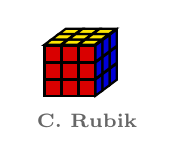
\begin{tikzpicture}[scale=0.6]
    \VeKhoiRubik{-0.7}{-0.7}
    \node[below=3pt, font=\scriptsize\bfseries\color{gray!80!black}] at (0.2,-0.7) {C. Rubik};
  \end{tikzpicture}
  &
  \begin{tikzpicture}[scale=0.6]
    \VeKhoiLapPhuong[orange!50]{-0.6}{-0.6}{1.1}
    \node[below=3pt, font=\scriptsize\bfseries\color{gray!80!black}] at (0,-0.6) {D. Hộp gỗ};
  \end{tikzpicture}
\end{tabular}
\end{center}
\choice
{Viên xúc xắc}
{Khối đồ chơi rubik}
{Hộp gỗ hình vuông}
{\True Hộp sữa tươi hình chữ nhật}
\loigiai{
Hộp sữa tươi có dạng khối hộp chữ nhật, không phải khối lập phương.\\
\textbf{Đáp án của câu hỏi là D}
}
\end{ex}

% --- CÂU 12 ---
\begin{ex} %[1H4C14]
Ghép 2 khối lập phương bằng nhau cạnh nhau như hình dưới đây, ta nhận được hình khối gì?
\begin{center}
\begin{tikzpicture}[scale=0.8, baseline=(current bounding box.center)]
  \VeKhoiLapPhuong[yellow!60]{-1.3}{-0.5}{1.1}
  \VeKhoiLapPhuong[cyan!50]{-0.2}{-0.5}{1.1}
  \node[below=4pt, font=\small\bfseries\color{blue!90!black}] at (0,-0.6) {2 khối lập phương ghép sát nhau};
\end{tikzpicture}
\end{center}
\choice
{Khối lập phương}
{Khối cầu}
{Khối trụ}
{\True Khối hộp chữ nhật}
\loigiai{
Ghép 2 khối lập phương bằng nhau liền kề tạo thành một \textbf{khối hộp chữ nhật}.\\
\textbf{Đáp án của câu hỏi là D}
}
\end{ex}

\newpage
% =========================================================================
% PHẦN 2: TRẮC NGHIỆM ĐÚNG SAI (2 CÂU)
% =========================================================================
\textbf{Phần 2. Trắc nghiệm đúng sai}
\setcounterpageref{ex}{0}

% --- CÂU 13 ---
\begin{ex} %[1H4H14]
Quan sát khối lập phương và khối hộp chữ nhật dưới đây:
\begin{center}
\setlength{\tabcolsep}{15pt}
\begin{tabular}{cc}
  \begin{tikzpicture}[scale=0.8]
    \VeKhoiLapPhuong[yellow!60]{-0.6}{-0.6}{1.2}
    \node[below=3pt, font=\small\bfseries\color{orange!90!black}] at (0,-0.6) {Khối lập phương};
  \end{tikzpicture}
  &
  \begin{tikzpicture}[scale=0.8]
    \VeKhoiHopChuNhat[cyan!50]{-1.0}{-0.6}{2.0}{1.2}{0.8}
    \node[below=3pt, font=\small\bfseries\color{blue!90!black}] at (0,-0.6) {Khối hộp chữ nhật};
  \end{tikzpicture}
\end{tabular}
\end{center}
Xét tính đúng sai của các câu sau:
\choiceTF
{\True Khối lập phương có 6 mặt đều là các hình vuông bằng nhau.}
{\True Khối hộp chữ nhật có 6 mặt.}
{Khối lập phương có 8 mặt phẳng.}
{\True Khối lập phương và khối hộp chữ nhật đều có 6 mặt.}
\loigiai{
\begin{itemize}
    \item a) \textbf{Đúng}: Khối lập phương có 6 mặt vuông bằng nhau.
    \item b) \textbf{Đúng}: Khối hộp chữ nhật có 6 mặt.
    \item c) \textbf{Sai}: Khối lập phương có 6 mặt, không phải 8 mặt.
    \item d) \textbf{Đúng}: Cả hai khối đều có đúng 6 mặt.
\end{itemize}
}
\end{ex}

% --- CÂU 14 ---
\begin{ex} %[1H4V14]
Mô hình ngôi nhà đồ chơi được bạn Nam ghép bởi các hình khối như sau:
\begin{center}
\begin{tikzpicture}[scale=0.8, baseline=(current bounding box.center)]
  \VeKhoiHopChuNhat[yellow!55]{-1.3}{-1.2}{2.4}{1.4}{1.0}
  \node[font=\footnotesize\bfseries\color{orange!90!black}] at (0,-0.5) {Thân nhà (khối HCN)};
  
  \VeKhoiLapPhuong[red!55]{-1.1}{0.5}{0.7}
  \node[left=3pt, font=\tiny\bfseries\color{red!85!black}] at (-1.1,0.85) {Ống khói (khối LP)};
\end{tikzpicture}
\end{center}
Xét tính đúng sai của các câu sau:
\choiceTF
{\True Thân ngôi nhà có dạng khối hộp chữ nhật.}
{\True Ống khói ngôi nhà có dạng khối lập phương.}
{Ngôi nhà được ghép bởi tất cả 5 hình khối.}
{\True Ngôi nhà gồm 1 khối hộp chữ nhật và 1 khối lập phương.}
\loigiai{
\begin{itemize}
    \item a) \textbf{Đúng}: Thân nhà là khối hộp chữ nhật.
    \item b) \textbf{Đúng}: Ống khói là khối lập phương.
    \item c) \textbf{Sai}: Ngôi nhà chỉ ghép bởi 2 khối (1 thân + 1 ống khói), không phải 5 khối.
    \item d) \textbf{Đúng}: Gồm đúng 1 khối hộp chữ nhật và 1 khối lập phương.
\end{itemize}
}
\end{ex}

% =========================================================================
% PHẦN 3: TRẢ LỜI NGẮN (6 CÂU)
% =========================================================================
\textbf{Phần 3. Trả lời ngắn (Quan sát hình vẽ và điền số thích hợp)}
\setcounterpageref{ex}{0}

% --- CÂU 15 ---
\begin{ex} %[1H4H14]
Khối lập phương có tất cả bao nhiêu mặt?
\begin{center}
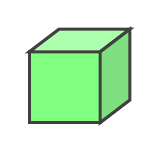
\begin{tikzpicture}[scale=0.75, baseline=(current bounding box.center)]
  \VeKhoiLapPhuong[green!50]{-0.6}{-0.6}{1.2}
\end{tikzpicture}
\end{center}
\shortans{6}
\loigiai{
\textbf{Đáp số:} $6$\\
Khối lập phương có $6$ mặt vuông bằng nhau.
}
\end{ex}

% --- CÂU 16 ---
\begin{ex} %[1H4H14]
Khối hộp chữ nhật có tất cả bao nhiêu mặt?
\begin{center}
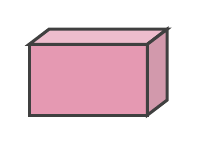
\begin{tikzpicture}[scale=0.75, baseline=(current bounding box.center)]
  \VeKhoiHopChuNhat[purple!40]{-1.0}{-0.6}{2.0}{1.2}{0.8}
\end{tikzpicture}
\end{center}
\shortans{6}
\loigiai{
\textbf{Đáp số:} $6$\\
Khối hộp chữ nhật có $6$ mặt.
}
\end{ex}

\newpage
% --- CÂU 17 ---
\begin{ex} %[1H4V14]
Bé xếp các khối lập phương thành hình bậc thang: tầng dưới cùng có 3 khối, tầng giữa có 2 khối, tầng trên cùng có 1 khối như hình vẽ. Hỏi có tất cả bao nhiêu khối lập phương?
\begin{center}
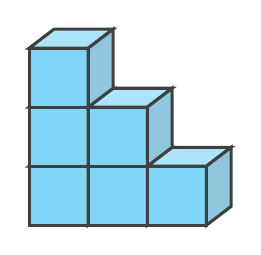
\begin{tikzpicture}[scale=0.75, baseline=(current bounding box.center)]
  % Tầng dưới: 3 khối
  \VeKhoiLapPhuong[cyan!50]{-1.5}{-1.2}{1.0}
  \VeKhoiLapPhuong[cyan!50]{-0.5}{-1.2}{1.0}
  \VeKhoiLapPhuong[cyan!50]{0.5}{-1.2}{1.0}
  % Tầng giữa: 2 khối
  \VeKhoiLapPhuong[cyan!50]{-1.5}{-0.2}{1.0}
  \VeKhoiLapPhuong[cyan!50]{-0.5}{-0.2}{1.0}
  % Tầng trên: 1 khối
  \VeKhoiLapPhuong[cyan!50]{-1.5}{0.8}{1.0}
\end{tikzpicture}
\end{center}
\shortans{6}
\loigiai{
\textbf{Đáp số:} $6$\\
Tổng số khối là: $3 + 2 + 1 = 6$ khối lập phương.
}
\end{ex}

% --- CÂU 18 ---
\begin{ex} %[1H4V14]
Bé có 4 khối hộp chữ nhật màu xanh và 3 khối lập phương màu đỏ. Hỏi bé có tất cả bao nhiêu khối đồ chơi?
\begin{center}
\begin{tikzpicture}[scale=0.7, baseline=(current bounding box.center)]
  \foreach \i in {0,1,2,3} {
    \VeKhoiHopChuNhat[cyan!50]{\i*1.5 - 4.5}{-0.5}{1.1}{0.8}{0.5}
  }
  \node[below=3pt, font=\small\bfseries\color{blue!90!black}] at (-2.3,-0.6) {4 khối hộp chữ nhật};
  
  \foreach \i in {0,1,2} {
    \VeKhoiLapPhuong[red!50]{\i*1.3 + 1.2}{-0.5}{0.9}
  }
  \node[below=3pt, font=\small\bfseries\color{red!85!black}] at (2.5,-0.6) {3 khối lập phương};
\end{tikzpicture}
\end{center}
\shortans{7}
\loigiai{
\textbf{Đáp số:} $7$\\
$4 + 3 = 7$ khối đồ chơi.
}
\end{ex}

% --- CÂU 19 ---
\begin{ex} %[1H4V14]
Khối lập phương lớn gồm 2 tầng, mỗi tầng có 4 khối lập phương nhỏ như hình vẽ. Hỏi có tất cả bao nhiêu khối lập phương nhỏ?
\begin{center}
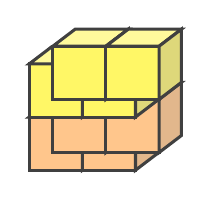
\begin{tikzpicture}[scale=0.75, baseline=(current bounding box.center)]
  % Tầng 1
  \VeKhoiLapPhuong[orange!45]{-0.9}{-0.9}{0.9}
  \VeKhoiLapPhuong[orange!45]{0}{-0.9}{0.9}
  \VeKhoiLapPhuong[orange!45]{-0.5}{-0.6}{0.9}
  \VeKhoiLapPhuong[orange!45]{0.4}{-0.6}{0.9}
  % Tầng 2
  \VeKhoiLapPhuong[yellow!60]{-0.9}{0}{0.9}
  \VeKhoiLapPhuong[yellow!60]{0}{0}{0.9}
  \VeKhoiLapPhuong[yellow!60]{-0.5}{0.3}{0.9}
  \VeKhoiLapPhuong[yellow!60]{0.4}{0.3}{0.9}
\end{tikzpicture}
\end{center}
\shortans{8}
\loigiai{
\textbf{Đáp số:} $8$\\
$4 + 4 = 8$ khối lập phương nhỏ.
}
\end{ex}

% --- CÂU 20 ---
\begin{ex} %[1H4C14]
Bạn Nam có 10 khối gỗ gồm khối lập phương và khối hộp chữ nhật. Trong đó có 6 khối lập phương. Hỏi Nam có bao nhiêu khối hộp chữ nhật?
\begin{center}
\begin{tikzpicture}[scale=0.8, baseline=(current bounding box.center)]
  \draw[fill=blue!6, draw=blue!70!black, line width=1.3pt, rounded corners=6pt] (-3.8,-0.6) rectangle (3.8,0.6);
  \node[font=\large\bfseries\color{blue!90!black}] at (0,0) {10 khối $-$ 6 khối lập phương = ? khối hộp chữ nhật};
\end{tikzpicture}
\end{center}
\shortans{4}
\loigiai{
\textbf{Đáp số:} $4$\\
$10 - 6 = 4$ khối hộp chữ nhật.
}
\end{ex}
